%%%%%%%%%%%%%%%%%%%%%%%%%%%%%%%%%%%%%%%%%%%%%%%%%%%%%%%%%%%%%%%%%%%%%%
% Lớp 10 | Véctơ (chưa xét tọa độ) | Tích của một số với véctơ
% Dạng 0H5?3-6: Tính độ dài của véctơ tổng, hiệu
% Số câu: 16  (sinh tự động bởi tach_cau.py; từ nay thầy sửa trực tiếp file này)
%%%%%%%%%%%%%%%%%%%%%%%%%%%%%%%%%%%%%%%%%%%%%%%%%%%%%%%%%%%%%%%%%%%%%%

%%%%%%%%%%%%%%%% TRẮC NGHIỆM 4 PHƯƠNG ÁN %%%%%%%%%%%%%%%%

% nguồn: MaHoaNH_TracNghiem_Lop10
\begin{ex}%[0H5V3-6]%[ma:11f2f6c8]
	Cho tam giác đều  $ABC$. Phát biểu nào sau đây đúng?
	 \choice
		{$\overrightarrow{AB}-\overrightarrow{BC}=\overrightarrow0$} 
		{\True  $\left|\overrightarrow{AB}\right|=\left|\overrightarrow{AC}\right|$}
		 {$\overrightarrow{AB}=\overrightarrow{AC}$}
		{$\overrightarrow{AB}+\overrightarrow{BC}=\overrightarrow{CA}$} 
	 \loigiai{
		Vì $\triangle  ABC$ đều nên $AB=AC\Rightarrow \left|\overrightarrow{AB}\right|=\left|\overrightarrow{AC}\right|$.
	 }
\end{ex}

% nguồn: MaHoaNH_TracNghiem_Lop10
\begin{ex}%[0H5V3-6]%[ma:6f50d32c]
	Trên trục tọa độ $\left(O; \overrightarrow{e}\right)$, các điểm $A, B$  và $C$ có tọa độ lần lượt là $-1$; $2$ và $3$. Tìm giá trị của $\overline{AB}+2\overline{AC}$.
	\choice 
		{\True $11$} 
		{$1$} 
		{$7$} 
		{$-11$} 
	\loigiai{ 
		\[\overline{AB}=2-\left(-1\right)=3, \overline{AC}=3-\left(-1\right)=4\Rightarrow \overline{AB}+2\overline{AC}=3+2\cdot4=11. 
		 \]
	} 
\end{ex}

% nguồn: MaHoaNH_TracNghiem_Lop10
\begin{ex}%[0H5V3-6]%[ma:2f55e4d5]
	Cho tam giác $ABC$, có bao nhiêu điểm $M$ thỏa  $\left|\overrightarrow{MA}+\overrightarrow{MB}+\overrightarrow{MC}\right|=5$?
	 \choice
		 {$1$}
		{$2$} 
		{\True  Vô số}
		{Không có  điểm nào}
	 \loigiai{
		Gọi $G$ là trọng tâm tam giác  $ABC$, ta có:
		$$\left|\overrightarrow{MA}+\overrightarrow{MB}+\overrightarrow{MC}\right|=5\Leftrightarrow  \left|3\overrightarrow{MG}\right|=5\Leftrightarrow MG=\dfrac{5}{3}
		$$ 
		Vậy quỹ tích điểm $M$ là đường  tròn tâm $G$, bán kính $\dfrac{5}{3}$.
	} 
\end{ex}

% nguồn: MaHoaNH_TracNghiem_Lop10
\begin{ex}%[0H5V3-6]%[ma:3a9a925b]
	Cho  tam giác $ABC$ đều cạnh bằng $1$. Ta có
	 \choice
		 {\True $\left|\overrightarrow{AB}-\overrightarrow{CA}\right|=\sqrt{3}$}
		 {$\left|\overrightarrow{AB}-\overrightarrow{CA}\right|=0$}
		 {$\left|\overrightarrow{AB}-\overrightarrow{CA}\right|=2$}
		{$\left|\overrightarrow{AB}-\overrightarrow{AC}\right|=0$} 
	 \loigiai{
	\immini{Gọi $M$ là trung điểm của $BC$ ta có $AM=\dfrac{\sqrt{3}}{2}$. Khi đó $\overrightarrow{AB}-\overrightarrow{CA}=\overrightarrow{AB}+\overrightarrow{AC}=2\overrightarrow{AM}$.\\ 
		Nên $\left|\overrightarrow{AB}-\overrightarrow{CA}\right|=\left|\overrightarrow{AB}+\overrightarrow{AC}\right|=2\left|\overrightarrow{AM}\right|=\sqrt{3}$.}{\begin{tikzpicture}[scale=0.7,font=\footnotesize,line join=round,line cap=round,>=stealth]
		\path  (0,0) coordinate (A)
			(0:4)  coordinate (B)
			(60:4)  coordinate (C)
			($(C)!0.5!(B)$) coordinate (M); 
		\draw[thick,->]  (A)--(B);
		\draw[thick,->]  (C)--(A);
		\draw[thick,->] (A)--(M); 
		\draw (B)--(C); 
		\foreach \x/\g in {A/180,M/60,B/0,C/90} \fill (\x) circle  (1.0pt)+(\g:.3) node {$\x$};
	\end{tikzpicture}
		 }
	} 
\end{ex}

% nguồn: MaHoaNH_TracNghiem_Lop10
\begin{ex}%[0H5V3-6]%[ma:3fa4786d]
	Cho  tam giác đều $ABC$ cạnh bằng $2a$. Khi đó $\left|\overrightarrow{AB}+\overrightarrow{AC}\right|$ bằng
	 \choice
		 {$a$}
		{\True $2\sqrt{3}  a$}
		{$\dfrac{\sqrt{3} a}{2}$} 
		{$2a$} 
	 \loigiai{
	\immini{  Ta có $\left|\overrightarrow{AB}+\overrightarrow{AC}\right|=\left|2\overrightarrow{AM}\right|=2.\dfrac{\sqrt{3}}{2}.2a=2\sqrt{3} a$.\\
		(với $M$ là trung điểm $BC$).}{\begin{tikzpicture}[scale=0.7,font=\footnotesize,line join=round,line cap=round,>=stealth]
		\path (0,0) coordinate  (A)
			 (0:4) coordinate (B)
			(60:4) coordinate  (C)
			($(C)!0.5!(B)$) coordinate  (M);
		\draw[thick,->] (A)--(B); 
		\draw[thick,->]  (A)--(C);
		\draw[thick,->]  (A)--(M);
		\draw (B)--(C); 
		\foreach \x/\g in {A/180,M/60,B/0,C/90} \fill (\x)  circle (1.0pt)+(\g:.3) node {$\x$};
	\end{tikzpicture}
		} 
	} 
\end{ex}

% nguồn: MaHoaNH_TracNghiem_Lop10
\begin{ex}%[0H5V3-6]%[ma:a79d8da2]
	Gọi $G$ là trọng tâm tam giác vuông $ABC$ với  cạnh huyền $BC=45$. Tính $\left|\overrightarrow{GB}+\overrightarrow{GC}\right|$?
	\choice 
		 {$45$}
		{$3\sqrt{5}$} 
		{\True $15$} 
		 {$30$}
	 \loigiai{
	\immini{Gọi $I$ là  trung điểm $BC$. Ta có\\ \[\left|\overrightarrow{GB}+\overrightarrow{GC}\right|=\left|2\overrightarrow{GI}\right|=\left|\dfrac{2}{3} \overrightarrow{AI}\right|=\dfrac{2}{3}\cdot \dfrac{BC}{2}=\dfrac{BC}{3}=15.
		\]}{\begin{tikzpicture}[scale=0.7,font=\footnotesize,line join=round,line cap=round,>=stealth]
		\path (0,0) coordinate (A) 
			(0:4)  coordinate (B)
			(90:4) coordinate  (C)
			 ($(C)!0.5!(B)$) coordinate (I)
			($(A)!2/3!(I)$)  coordinate (G);
		 \draw[thick,->] (G)--(B);
		\draw[thick,->]  (G)--(C);
		\draw[thick,->] (G)--(I); 
		\draw[thick,->]  (A)--(I);
		\draw (A)--(B)--(C)--(A); 
		\foreach  \x/\g in {A/180,I/60,B/0,C/180,G/-90} \fill (\x) circle (1.0pt)+(\g:.3) node {$\x$};
		\foreach \x/\y/\z  in {C/A/B}{\draw pic[draw,angle radius=2mm]{right angle=\x--\y--\z};}
	\end{tikzpicture}
		 }
	 }
\end{ex}

% nguồn: MaHoaNH_TracNghiem_Lop10
\begin{ex}%[0H5V3-6]%[ma:c90dea47]
	Cho tam giác $OAB$ vuông cân  tại $O$, $OA=a$, độ dài vectơ $3\overrightarrow{OA}+4\overrightarrow{OB}$ là
	\choice 
		 {\True $5a$}
		{$4a$} 
		{$7a$} 
		 {$a$}
	 \loigiai{
	\immini{ Đặt $\overrightarrow{OD}=3\overrightarrow{OA},  \overrightarrow{OE}=4\overrightarrow{OB}$.\\
		Lấy $C$ sao cho $DOEC$ là hình chữ nhật. Theo quy tắc cộng  hình bình hành thì $\overrightarrow{OD}+\overrightarrow{OE}=\overrightarrow{OC}$.\\
		Vậy $\left|\overrightarrow{OD}+\overrightarrow{OE}\right|=5a.$}{\begin{tikzpicture}[scale=0.5,font=\footnotesize,line join=round,line cap=round,>=stealth]
		 \path (0,0) coordinate [label=left:$O$](O)
			 (2,0) coordinate [label=below:$B$](B)
			(0,2)  coordinate [label=left:$A$](A)
			(8,0)  coordinate [label=below:$E$](E)
			(0,6) coordinate  [label=above:$D$](D)
			(8,6)  coordinate [label=above:$C$](C);
		 \draw[thick,->] (O)--(A);
		\draw[thick,->] (O)--(B); 
		\draw[thick,->]  (O)--(D);
		\draw[thick,->]  (O)--(C);
		\draw[thick,->]  (O)--(E);
		 \draw (E)--(C)--(D);
		\foreach \x/\y/\z in {D/O/E}{\draw pic[draw,angle radius=2mm]{right angle=\x--\y--\z};} 
	\end{tikzpicture}
		 }
	 }
\end{ex}

% nguồn: MaHoaNH_TracNghiem_Lop10
\begin{ex}%[0H5V3-6]%[ma:ef5d8737]
	Cho tam giác $ABC$ vuông cân  tại $A$, $AB=a$. Tính độ dài vectơ $\overrightarrow{AB}+4\overrightarrow{AC}$.
	\choice 
		{$\sqrt{20} a$} 
		{$5a$} 
		 {$17a$}
		 {\True $\sqrt{17} a$}
	 \loigiai{
	\immini{ Dựng các điểm $D$, $E$ sao cho $\overrightarrow{AD}=4\overrightarrow{AC}$ và tứ giác $ABED$ là hình  bình hành.\\
		 Khi đó $\left|\overrightarrow{AB}+4\overrightarrow{AC}\right|=\left|\overrightarrow{AB}+\overrightarrow{AD}\right|=\left|\overrightarrow{AE}\right|$.\\
		Áp dụng định lý Pi-ta-go cho tam giác $ADE$ ta  có\\
		$\left|\overrightarrow{AB}+4\overrightarrow{AC}\right|=\sqrt{a^2+(4a)^2}=a\sqrt{17}$.	}{\begin{tikzpicture}[scale=0.7,font=\footnotesize,line join=round,line cap=round,>=stealth]
		\path (0,0) coordinate  (A)
			(0:2) coordinate  (C)
			 (90:2) coordinate (B)
			(8,0)  coordinate (D)
			(8,2) coordinate (E); 
		\draw[thick,->] (A)--(B); 
		\draw[thick,->] (A)--(C); 
		\draw[thick,->] (A)--(D); 
		 \draw[thick,->] (A)--(E);
		\draw  (C)--(B)--(E)--(D);
		\foreach \x/\g in {A/-90,E/0,B/180,C/-90,D/-90} \fill (\x) circle (1.0pt)+(\g:.3) node  {$\x$};
		\foreach  \x/\y/\z in {B/A/D}{\draw pic[draw,angle radius=2mm]{right angle=\x--\y--\z};}
	\end{tikzpicture}
		} 
	 }
\end{ex}

% nguồn: MaHoaNH_TracNghiem_Lop10
\begin{ex}%[0H5V3-6]%[ma:3b29370b]
	Cho hình bình hành $ABCD$ có $AB=a$, $AB\perp BD$, $\widehat{BAD}=60^\circ$. Gọi $E$, $F$ lần lượt là trung điểm của $BD$, $AD$. Độ dài của vectơ  $\overrightarrow{BE}+\overrightarrow{AF}$ là
	 \choice
		{\True $\dfrac{a\sqrt{13}}{2}$} 
		 {$\dfrac{a\sqrt{10}}{2}$}
		{$\dfrac{a\sqrt{7}}{2}$} 
		{$2a$} 
	 \loigiai{
	\immini{Gọi $G$, $H$ lần lượt là trung điểm $AB$  và $EF$. Ta có $$BD=a\cdot\tan 60^o=a\sqrt{3}.$$ $GD=\sqrt{BD^2+BG^2}=\sqrt{\dfrac{a^2}{4}+3a^2}=\dfrac{a\sqrt{13}}{2}$.\\
		 $\overrightarrow{BE}+\overrightarrow{AF}=-(\overrightarrow{DE}+\overrightarrow{DF})=-2\overrightarrow{DH}=-\overrightarrow{DG}$.\\
		 Do đó $\left|\overrightarrow{BE}+\overrightarrow{AF}\right|=DG=\dfrac{a\sqrt{13}}{2}.
		$}{\begin{tikzpicture}[scale=0.7,font=\footnotesize,line join=round,line cap=round,>=stealth]
		\path  (0,0) coordinate (A)
			 (0:4) coordinate (B)
			(-60:8) coordinate  (D)
			($(B)+(D)-(A)$)  coordinate (C)
			 ($(D)!0.5!(B)$) coordinate (E)
			($(D)!0.5!(A)$)  coordinate (F)
			($(A)!0.5!(B)$)  coordinate (G)
			($(E)!0.5!(F)$) coordinate (H); 
		\draw[thick,->]  (B)--(E);
		\draw[thick,->] (A)--(F); 
		\draw  (A)--(B)--(C)--(D)--(F)--(E)--(D)--(G);
		\foreach \x/\g in {A/90,E/0,F/-150,B/90,C/0,G/90,H/70,D/-90} \fill (\x) circle (1.0pt)+(\g:.3) node  {$\x$};
	\end{tikzpicture}
		} 
	} 
\end{ex}

% nguồn: MaHoaNH_TracNghiem_Lop10
\begin{ex}%[0H5V3-6]%[ma:5fc1e72e]
	Cho tam giác $ABC$ đều có cạnh $AB=5$, $H$ là trung điểm  của $BC$. Tính $\left|\overrightarrow{CA}-\overrightarrow{HC}\right|$.
	\choice 
		 {$\left|\overrightarrow{CA}-\overrightarrow{HC}\right|=\dfrac{5\sqrt{3}}{2}$}
		 {$\left|\overrightarrow{CA}-\overrightarrow{HC}\right|=5$}
		{$\left|\overrightarrow{CA}-\overrightarrow{HC}\right|=\dfrac{5\sqrt{7}}{4}$} 
		 {\True $\left|\overrightarrow{CA}-\overrightarrow{HC}\right|=\dfrac{5\sqrt{7}}{2}$}
	\loigiai{ 
	\immini{ Ta  có $\left|\overrightarrow{CA}-\overrightarrow{HC}\right|=\left|\overrightarrow{CA}+\overrightarrow{CH}\right|=\left|2\overrightarrow{CE}\right|=2CE$ (với $E$ là trung điểm của $AH$.\\
		Ta lại có $AH=\dfrac{5\sqrt{3}}{2}$ ($\triangle ABC$ đều, $AH$ là  đường cao).\\
		Trong tam giác $HEC$ vuông tại $H$, có 
		\[EC=\sqrt{CH^2+HE^2}=\sqrt{2{,}5^2+\left(\dfrac{5\sqrt{3}}{4} \right)^2}=\dfrac{5\sqrt{7}}{4} \Rightarrow \left|\overrightarrow{CA}-\overrightarrow{HC}\right|=2CE=\dfrac{5\sqrt{7}}{2}. 
		\]}{\begin{tikzpicture}[scale=0.7,font=\footnotesize,line join=round,line cap=round,>=stealth]
		\path (0,0)  coordinate (A)
			(0:4)  coordinate (B)
			 (60:4) coordinate (C)
			($(C)!0.5!(B)$) coordinate (H) 
			 ($(H)!0.5!(A)$) coordinate (E);
		 \draw[thick,->] (C)--(A);
		 \draw[thick,->] (H)--(C);
		\draw[thick,->]  (C)--(E);
		 \draw (C)--(A)--(B)--(C)
			 (A)--(H);
		\foreach \x/\g in  {A/180,B/0,C/90,H/40,E/-90} \fill (\x) circle (1.0pt)+(\g:.3) node {$\x$};
	\end{tikzpicture}
		 }
	} 
\end{ex}

% nguồn: MaHoaNH_TracNghiem_Lop10
\begin{ex}%[0H5V3-6]%[ma:264c579e]
	Cho hình chữ nhật $ABCD$ có $AB=4a$ và $AD=3a$. Độ dài của vectơ $\overrightarrow{BA}+\overrightarrow{DA}$  bằng
	 \choice
		{\True  $5a$}
		 {$6a$}
		{$2a\sqrt{3}$} 
		{$7a$} 
	 \loigiai{
	\immini{Từ $B$ kẻ  $\overrightarrow{BE}=\overrightarrow{DA}$.\\
		Áp dụng quy tắc hình  hình hành: $\overrightarrow{BA}+\overrightarrow{DA}=\overrightarrow{BA}+\overrightarrow{BE}=\overrightarrow{BF}$ (với $F$ là đỉnh thứ tư của hình chữ nhật $ABEF$).\\
		Vậy $\left|\overrightarrow{BF}\right|=\sqrt{(4a)^2+(3a)^2}=5a. 
		$}{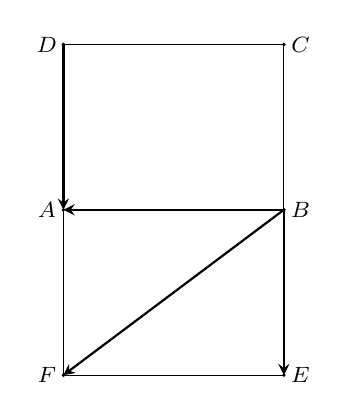
\begin{tikzpicture}[scale=0.7,font=\footnotesize,line join=round,line cap=round,>=stealth]
		\path (0,0) coordinate (A) 
			 (4,0) coordinate (B)
			 (0,3) coordinate (D)
			(4,3) coordinate (C) 
			(4,-3) coordinate (E) 
			(0,-3) coordinate (F); 
		\draw[thick,->] (B)--(A); 
		\draw[thick,->] (D)--(A); 
		\draw[thick,->]  (B)--(E);
		\draw[thick,->] (B)--(F); 
		\draw (E)--(F)--(A) 
			 (D)--(C)--(B);
		\foreach \x/\g in {A/180,D/180,F/180,E/0,B/0,C/0} \fill (\x) circle (1.0pt)+(\g:.3)  node {$\x$};
	\end{tikzpicture}
		} 
	 }
\end{ex}

% nguồn: MaHoaNH_TracNghiem_Lop10
\begin{ex}%[0H5V3-6]%[ma:2ac32b2b]
	Cho $\triangle ABC$ đều cạnh $a$, gọi $H$ là trung điểm  của cạnh $BC$. Tính $\left|\overrightarrow{CA}-\overrightarrow{HC}\right|$.
	 \choice
		{\True $\dfrac{\sqrt{7}  a}{2}$}
		{$\dfrac{a\sqrt{7}}{4}$} 
		 {$\dfrac{2\sqrt{3} a}{3}$}
		{$\dfrac{a}{2}$} 
	 \loigiai{
	\immini{ Gọi $D$ là  điểm thỏa mãn $\overrightarrow{AD}=\overrightarrow{CH}$. Khi đó $$\left|\overrightarrow{CA}-\overrightarrow{HC}\right|=\left|\overrightarrow{CA}+\overrightarrow{CH}\right|=\left|\overrightarrow{CD}\right|=CD.$$
		Ta thấy, $\overrightarrow{AD}=\overrightarrow{HB}$ vì $\overrightarrow{CH}=\overrightarrow{HB}$ (do $H$  trung điểm $BC$).\\
		Suy ra, $AHBD$ là hình bình hành. Mà $AH\perp BC$ (vì $\triangle ABC$ đều). Vậy $AHBD$  là hình chữ nhật.\\
		Suy  ra, $BD\perp BC$ và $BD=AH=\dfrac{a\sqrt{3}}{2}$.\\
		Áp dụng định lí Py-ta-go vào $\triangle DBC$ vuông tại  $B$, có\\
		 $$CD^2=BD^2+BC^2=\dfrac{3a^2}{4}+a^2=\dfrac{7a^2}{4} \Rightarrow CD=\dfrac{a\sqrt{7}}{2}.$$
		}{\begin{tikzpicture}[scale=0.7,font=\footnotesize,line join=round,line cap=round,>=stealth]
		 \path (0,0) coordinate (A)
			(0:4) coordinate  (B)
			 (60:4) coordinate (C)
			(-60:2) coordinate  (D)
			 ($(C)!0.5!(B)$) coordinate (H)
			($(H)!0.5!(A)$) coordinate (E); 
		\draw[thick,->] (C)--(A); 
		\draw[thick,->] (H)--(C); 
		 \draw[thick,->] (H)--(B);
		 \draw[thick,->] (A)--(D);
		 \draw (C)--(A)--(B)--(C)
			(A)--(H) 
			(B)--(D)--(C); 
		\foreach \x/\g in {A/180,B/0,C/90,H/40,D/-90} \fill (\x)  circle (1.0pt)+(\g:.3) node {$\x$};
	\end{tikzpicture}
		} 
		\noindent 
		 Vậy $\left|\overrightarrow{CA}-\overrightarrow{HC}\right|=CD=\dfrac{a\sqrt{7}}{2}$.
	 }
\end{ex}


%%%%%%%%%%%%%%%% ĐÚNG/SAI %%%%%%%%%%%%%%%%

% nguồn: MaHoaNH_DungSai_Lop10
\begin{ex}%[0H5H3-6]%[ma:940ff6d3]
	Cho tam giác đều $ABC$ có cạnh $AB=2a$. $G$ là trọng tâm tam giác $ABC$. $H$ là hình chiếu của $A$ xuống cạnh $BC$. Xét tính đúng sai của các mệnh  đề sau
	 \choiceTF
		 {$|2\overrightarrow{BC}|=2a$}
		{\True  $|-\overrightarrow{AC}|=2a$}
		{$|\overrightarrow{AG}|=\dfrac{2}{3}a$} 
		{\True $|\overrightarrow{AH}|=a\sqrt{3}$} 
	\loigiai{ 
		\begin{itemchoice}
			\itemch Ta  có $|2\overrightarrow{AB}|=2\cdot 2a=4a$.
			\itemch Ta có $|-\overrightarrow{AC}|=AC=2a$. 
			\itemch Ta có $|\overrightarrow{AG}|=\dfrac{2}{3}\cdot  \dfrac{2a\sqrt3}{2}=\dfrac{2a\sqrt{3}}{3}$.
			\itemch Ta có  $|\overrightarrow{AH}|= \dfrac{2a\sqrt3}{2}=a\sqrt3$.
		\end{itemchoice}
	 }
\end{ex}

% nguồn: MaHoaNH_DungSai_Lop10
\begin{ex}%[0H5H3-6]%[ma:0df721ae]
	Cho  hình chữ nhật $ABCD$ có $AB=3a$, $BC=4a$. Xét tính đúng sai của các mệnh đề sau
	 \choiceTF
		{\True $|5\overrightarrow{AB}|=15a$} 
		{$|3\overrightarrow{AC}|=12a$} 
		 {$|\overrightarrow{AB}+\overrightarrow{AD}|=15a$}
		{\True $|2\overrightarrow{AB}+\overrightarrow{AD}|=2a\sqrt{13}$} 
	\loigiai{ 
		\begin{itemchoice}
			\itemch Ta  có $|5\overrightarrow{AB}|=5\cdot 3a=15a$.
			\itemch Ta  có $AC=\sqrt{AB^2+BC^2}=\sqrt{(3a)^2+(4a)^2}=5a$. Do đó $|3\overrightarrow{AC}|=15a$.
			\itemch Ta  có $|\overrightarrow{AB}+\overrightarrow{AD}|=|\overrightarrow{AC}|=5a$.
			\itemch Lấy điểm $E$ sao cho $B $ là trung điểm của $AE$. Khi đó  $|2\overrightarrow{AB}+\overrightarrow{AD}|=|\overrightarrow{AE}+\overrightarrow{AD}|=|DE|=2a\sqrt{13}$.
			\begin{center}\begin{tikzpicture}[>=stealth,line join=round,line cap=round,font=\footnotesize,scale=0.8]
		\def\d{4} 
		 \def\r{3}
		\path  (0:0) coordinate (B)
			++(0:\d)  coordinate (C)
			 ++(90:\r) coordinate (D)
			 ++(180:\d) coordinate (A)
			($(A)!2!(B)$)  coordinate (E);
		\draw (A)--(B)--(C)--(D)--cycle  (A)--(E)
			 (D)--(E);
		\foreach \x/ \goc  in {A/135,B/-135,C/-45,D/45,E/0}
		\fill  (\x) circle (1pt)
			($(\x)+(\goc:3mm)$) node {$\x$}; 
	\end{tikzpicture}
			\end{center}
		\end{itemchoice}
	} 
\end{ex}


%%%%%%%%%%%%%%%% TRẢ LỜI NGẮN %%%%%%%%%%%%%%%%

% nguồn: MaHoaNH_TraLoiNgan_Lop10
\begin{bt}%[0H5H3-6]%[ma:576d5677]
	Cho $\triangle ABC$ vuông tại $B$ có $\widehat{A}=30^{\circ}, AB = \sqrt{3}$. Gọi $I$ là trung điểm của $AC$. Giá trị của  $\left|\overrightarrow{BA}+\overrightarrow{BC}\right|$ bằng bao nhiêu?
	 \shortans{2}
	 \loigiai{
	 \immini{
		Xét $\triangle ABC$  vuông tại $B$ có $\tan A=\dfrac{BC}{AB} $\\$\Rightarrow BC=AB\cdot \tan A=\sqrt{3} \tan 30^{\circ}=1$.\\
		$AC=\sqrt{A B^2+BC^2}=\sqrt{3+1}=2$.\\ 
		Suy ra $\left| \overrightarrow{BA}+\overrightarrow{BC}\right|=\left|  2 \overrightarrow{B I}\right|=2\left| \overrightarrow{B I}\right|=2 B I=2 \cdot \dfrac{AC}{2}=AC=2$.
		 }{
		\begin{tikzpicture}[scale=1,font=\footnotesize,line join=round,line cap=round,>=stealth]
				\path (0,0) coordinate (B)++(0:3.46)  coordinate (A)
					($(B)+(90:2)$) coordinate (C) 
					($(A)!1/2!(C)$) coordinate (I); 
				 \draw (A)--(B)--(C)--(A)
					 (B)--(I);
				\foreach \x/\g in {A/0,B/-150,C/90,I/60} \fill (\x) circle (1.2pt)+(\g:.3) node  {$\x$};
				\foreach \x/\y/\z in {C/B/A}{\draw pic[draw,angle radius=2mm]{right angle=\x--\y--\z};} 
			\end{tikzpicture}
		 }
	 }
\end{bt}


%%%%%%%%%%%%%%%% TỰ LUẬN %%%%%%%%%%%%%%%%

% nguồn: MaHoaNH_TuLuan_Lop10
\begin{bt}%[0H5H3-6]%[ma:28874cf6]
	Cho tứ giác  $ABCD$. Gọi $I$, $J$ theo thứ tự là trung điểm của $AB$, $CD$ và $IJ=\dfrac{5}{4}$.Gọi $M$, $N$ theo thứ tự là trung điểm của $BC$, $AC$. Tính giá trị của biểu thức $\left|\overrightarrow{AM}+\overrightarrow{BN}+\overrightarrow{CJ}\right|$.
	 \loigiai{
	 \immini{
		Theo tính chất trung điểm ta có $\heva{ & 2 \overrightarrow{AM}=\overrightarrow{AB}+\overrightarrow{AC} \\ 
		 & 2 \overrightarrow{BN}=\overrightarrow{B A}+\overrightarrow{BC}\\
		& 2\overrightarrow{CI}=\overrightarrow{CA}+\overrightarrow{CB}. 
		 }$\\
		Cộng ba đẳng thức  trên ta được
		 \allowdisplaybreaks
		\begin{eqnarray*}
			&&2\left(\overrightarrow{AM}+\overrightarrow{B  N}+\overrightarrow{C I}\right)\\&=&\left(\overrightarrow{AB}+\overrightarrow{B A}\right)+\left(\overrightarrow{AC}+\overrightarrow{C A}\right)+\left(\overrightarrow{BC}+\overrightarrow{C B}\right)\\&=&\overrightarrow{0}.
		\end{eqnarray*}
		Suy ra $\overrightarrow{AM}+\overrightarrow{BN}+\overrightarrow{CJ}  = \overrightarrow{AM}+\overrightarrow{BN}+\overrightarrow{CI} + \overrightarrow{IJ}=\overrightarrow{0} +\overrightarrow{IJ} = \overrightarrow{IJ}$.\\
		Do vậy $\left|\overrightarrow{AM}+\overrightarrow{BN}+\overrightarrow{CJ}\right|=\left|\overrightarrow{IJ}\right| = \dfrac{5}{4}$. 
		}{ 
		\begin{tikzpicture}[scale=0.8,font=\footnotesize,line join=round,line cap=round,>=stealth]
				\path (0,0)  coordinate (A)++(0:4) coordinate (B)++(120:4) coordinate (C)++(-150:2) coordinate (D)
					($(B)!1/2!(A)$)  coordinate (I)
					 ($(C)!1/2!(D)$) coordinate (J)
					($(C)!1/2!(B)$) coordinate (M) 
					($(C)!1/2!(A)$) coordinate  (N);
				\draw  (A)--(B)--(C)--(D)--(A)--(C)
					(A)--(M) 
					(B)--(N) 
					(C)--(I); 
				\foreach  \x/\g in {A/-150,B/-20,C/90,D/120,I/-90,J/120,M/10,N/160} \fill (\x) circle (1.2pt)+(\g:.3) node {$\x$};
			\end{tikzpicture}
		} 
	} 
\end{bt}
